
\textit{Available users} are those for which user profile data was successfully collected.  Unavailable users are those for whom an attempt to acquire user attributes resulted in a \textit{404 Not Found} error.  We assume these user accounts are closed.\\

\begin{tabular}[t]{| l | l | l | l | l | l |}
\hline
& \textbf{Total} & \textbf{\# Available} & \textbf{\% Available} & \textbf{\# Unavailable} & \textbf{\% Unavailable} \\ \hline
\textbf{All} & 17,688,493 & 17,475,570 & 98.8\% & 212,923 & 1.2\% \\ \hline
\textbf{Core} & 242,275 & 238,323 & 98.8\% & 3,952 & 1.2\% \\ \hline
\textbf{Connected} & 15,548,091 & & & & \\ \hline
\textbf{Random} & & & & & \\ \hline
\end{tabular}

\subsection{Subgraphs}
\textit{Graph edges} refers to the connections between core users and any other user.\\

\begin{tabular}{| l | l | }
\hline
Users is Subgraph 1 & 15,548,091 \\ \hline
Available Users is Subgraph 1 & 15,363,277 \\ \hline
Core Users in Subgraph 1  & 194,004 \\ \hline
Remaining Core Users  & 48,267 \\ \hline
Remaining Subgraphs  & 46,403 \\ \hline
Connections to Subgraph 1  & 46,924 \\ \hline
Total Connected Users & 240,932 \\ \hline
\end{tabular}

\subsection{Boolean User Attributes}
Attributes whose values are either \textit{true} or \textit{false}.\\

\begin{tabular}{| l | l | l |}
\hline
\textbf{Attribute} & \textbf{\# True (Core)} & \textbf{\% True (Core)} \\ \hline
Protected & 8,517 & 3.575  \\ \hline
Geo-Enabled & 58,432 & 24.518 \\ \hline
Verified & 119 & 0.050 \\ \hline
Contributors Enabled & 7 & 0.003 \\ \hline
Show All Inline Media & 18,870 & 7.918 \\ \hline
URL & 118,364 & 49.665 \\ \hline
Is Translator & 72 & 0.030 \\ \hline
\end{tabular}

\subsection{Enumerated User Attributes}
Attributes for which there are a relatively small number of values, other than boolean values.
\subsubsection{Language}
Percentage of users per language.\\

\begin{tabular}{| l | l | l | l | l | l | l | l |}
\hline
\textbf{Language Code} & \textbf{Language} & \textbf{\# (All)}  & \textbf{\% (All)} & \textbf{\# (Core)}  & \textbf{\% (Core)} & \textbf{\# (Random)} & \textbf{\% (Random)} \\ \hline
en & English & 11,553,068 & 78.996 & 173,782 & 72.919 & & \\ \hline
es & Spanish & 1,426,063 & 9.751 & 16,210 & 6.802 & & \\ \hline
ja & Japanese & 1,360,341 & 9.302 & 44,499 & 18.672 & & \\ \hline
fr & French & 111,423 & 0.762 & 1,222 & 0.513 & & \\ \hline
de & German & 107,880 & 0.738 & 1,560 & 0.655 & & \\ \hline
it & Italian & 54,948 & 0.376 & 713 & 0.299 & & \\ \hline
ko & Korean & 11,114 & 0.076 & 337 & 0.141 & & \\ \hline
\end{tabular}

\subsubsection{UTC Offset}
Time zone, which appears later in this document, is essentially UTC offset data with redundancy -- some time zones have the same UTC offset.\\\\
\begin{tabular}{| l | l | l |}
\hline
\textbf{UTC Offset} & \textbf{\# (Core)} & \textbf{\% (Core)} \\ \hline
(none)	&	38287	&	16.065	\\ \hline
32400	&	36551	&	15.337	\\ \hline
-18000	&	26196	&	10.992	\\ \hline
-10800	&	25001	&	10.490	\\ \hline
-28800	&	23344	&	9.795	\\ \hline
-21600	&	17830	&	7.481	\\ \hline
-14400	&	12698	&	5.328	\\ \hline
25200	&	10425	&	4.374	\\ \hline
-36000	&	10162	&	4.264	\\ \hline
3600	&	9607	&	4.031	\\ \hline
0	&	7067	&	2.965	\\ \hline
-25200	&	4360	&	1.829	\\ \hline
28800	&	4065	&	1.706	\\ \hline
-32400	&	3573	&	1.499	\\ \hline
-16200	&	2685	&	1.127	\\ \hline
7200	&	1908	&	0.801	\\ \hline
36000	&	1286	&	0.540	\\ \hline
10800	&	1054	&	0.442	\\ \hline
19800	&	717	&	0.301	\\ \hline
43200	&	322	&	0.135	\\ \hline
-39600	&	236	&	0.099	\\ \hline
14400	&	213	&	0.089	\\ \hline
18000	&	163	&	0.068	\\ \hline
12600	&	138	&	0.058	\\ \hline
34200	&	103	&	0.043	\\ \hline
-7200	&	100	&	0.042	\\ \hline
21600	&	91	&	0.038	\\ \hline
-12600	&	57	&	0.024	\\ \hline
46800	&	24	&	0.010	\\ \hline
-3600	&	20	&	0.008	\\ \hline
39600	&	19	&	0.008	\\ \hline
16200	&	9	&	0.004	\\ \hline
23400	&	7	&	0.003	\\ \hline
20700	&	5	&	0.002	\\ \hline
\end{tabular}
\vspace{2.5in}

\subsubsection{Time Zone}
Only the top 100 time zones are shown here.\\
\begin{tabular}{| l | l | l | l | l | l |}
\hline
\textbf{Time Zone} & \textbf{\# (Core)} & \textbf{\% (Core)} & \textbf{Time Zone} & \textbf{\# (Core)} & \textbf{\% (Core)} \\ \hline
(none)	&	38287	&	16.065	&	Kyiv	&	215	&	0.090	\\ \hline
Tokyo	&	30332	&	12.727	&	Brussels	&	214	&	0.090	\\ \hline
Pacific Time (US \& Canada)	&	23280	&	9.768	&	Monterrey	&	214	&	0.090	\\ \hline
Brasilia	&	15997	&	6.712	&	Lima	&	194	&	0.081	\\ \hline
Central Time (US \& Canada)	&	15327	&	6.431	&	Copenhagen	&	183	&	0.077	\\ \hline
Eastern Time (US \& Canada)	&	15066	&	6.322	&	Riyadh	&	178	&	0.075	\\ \hline
Santiago	&	12131	&	5.090	&	Abu Dhabi	&	173	&	0.073	\\ \hline
Hawaii	&	10162	&	4.264	&	Athens	&	164	&	0.069	\\ \hline
Quito	&	10152	&	4.260	&	Bucharest	&	151	&	0.063	\\ \hline
Jakarta	&	9334	&	3.917	&	West Central Africa	&	151	&	0.063	\\ \hline
Greenland	&	7968	&	3.343	&	Warsaw	&	148	&	0.062	\\ \hline
London	&	5968	&	2.504	&	Perth	&	145	&	0.061	\\ \hline
Mountain Time (US \& Canada)	&	3826	&	1.605	&	Chennai	&	144	&	0.060	\\ \hline
Amsterdam	&	3600	&	1.511	&	Auckland	&	139	&	0.058	\\ \hline
Alaska	&	3573	&	1.499	&	Tehran	&	138	&	0.058	\\ \hline
Osaka	&	3509	&	1.472	&	Guadalajara	&	133	&	0.056	\\ \hline
Caracas	&	2685	&	1.127	&	Cairo	&	130	&	0.055	\\ \hline
Seoul	&	1912	&	0.802	&	Vienna	&	126	&	0.053	\\ \hline
Mexico City	&	1829	&	0.767	&	Wellington	&	124	&	0.052	\\ \hline
Singapore	&	1677	&	0.704	&	Kuwait	&	122	&	0.051	\\ \hline
Berlin	&	1494	&	0.627	&	Jerusalem	&	117	&	0.049	\\ \hline
Madrid	&	1160	&	0.487	&	Budapest	&	115	&	0.048	\\ \hline
Paris	&	1106	&	0.464	&	Bern	&	114	&	0.048	\\ \hline
Buenos Aires	&	1008	&	0.423	&	Mid-Atlantic	&	100	&	0.042	\\ \hline
Bangkok	&	1000	&	0.420	&	Helsinki	&	96	&	0.040	\\ \hline
Kuala Lumpur	&	944	&	0.396	&	Riga	&	93	&	0.039	\\ \hline
Sapporo	&	762	&	0.320	&	Adelaide	&	91	&	0.038	\\ \hline
Hong Kong	&	627	&	0.263	&	Hanoi	&	73	&	0.031	\\ \hline
Moscow	&	595	&	0.250	&	St. Petersburg	&	73	&	0.031	\\ \hline
Rome	&	594	&	0.249	&	Belgrade	&	71	&	0.030	\\ \hline
Sydney	&	562	&	0.236	&	Nairobi	&	66	&	0.028	\\ \hline
Bogota	&	526	&	0.221	&	Tijuana	&	64	&	0.027	\\ \hline
Istanbul	&	474	&	0.199	&	Casablanca	&	63	&	0.026	\\ \hline
Arizona	&	455	&	0.191	&	Ekaterinburg	&	63	&	0.026	\\ \hline
Edinburgh	&	411	&	0.172	&	Prague	&	62	&	0.026	\\ \hline
Beijing	&	399	&	0.167	&	Newfoundland	&	57	&	0.024	\\ \hline
Melbourne	&	396	&	0.166	&	Minsk	&	54	&	0.023	\\ \hline
Dublin	&	362	&	0.152	&	Sofia	&	51	&	0.021	\\ \hline
Stockholm	&	357	&	0.150	&	Islamabad	&	49	&	0.021	\\ \hline
Atlantic Time (Canada)	&	339	&	0.142	&	Kolkata	&	49	&	0.021	\\ \hline
New Delhi	&	304	&	0.128	&	Canberra	&	48	&	0.020	\\ \hline
Central America	&	301	&	0.126	&	Fiji	&	46	&	0.019	\\ \hline
Pretoria	&	275	&	0.115	&	Chihuahua	&	44	&	0.018	\\ \hline
Indiana (East)	&	258	&	0.108	&	Harare	&	44	&	0.018	\\ \hline
Lisbon	&	243	&	0.102	&	Karachi	&	43	&	0.018	\\ \hline
Taipei	&	231	&	0.097	&	Zagreb	&	39	&	0.016	\\ \hline
La Paz	&	228	&	0.096	&	Yakutsk	&	36	&	0.015	\\ \hline
Brisbane	&	225	&	0.094	&	Mazatlan	&	35	&	0.015	\\ \hline
Mumbai	&	220	&	0.092	&	Novosibirsk	&	32	&	0.013	\\ \hline
International Date Line West	&	216	&	0.091	&	Georgetown	&	28	&	0.012	\\ \hline
\end{tabular}

\subsubsection{Status Source}
Source of the most recent tweet.  Only the top 50 sources are included here.  We have not decided what to do with this information.  One problem with this data is that it is per-tweet.  That is, a user could have multiple tweet locations, and we are not capturing that data.  These are only the sources of the most recent tweets.\\\\
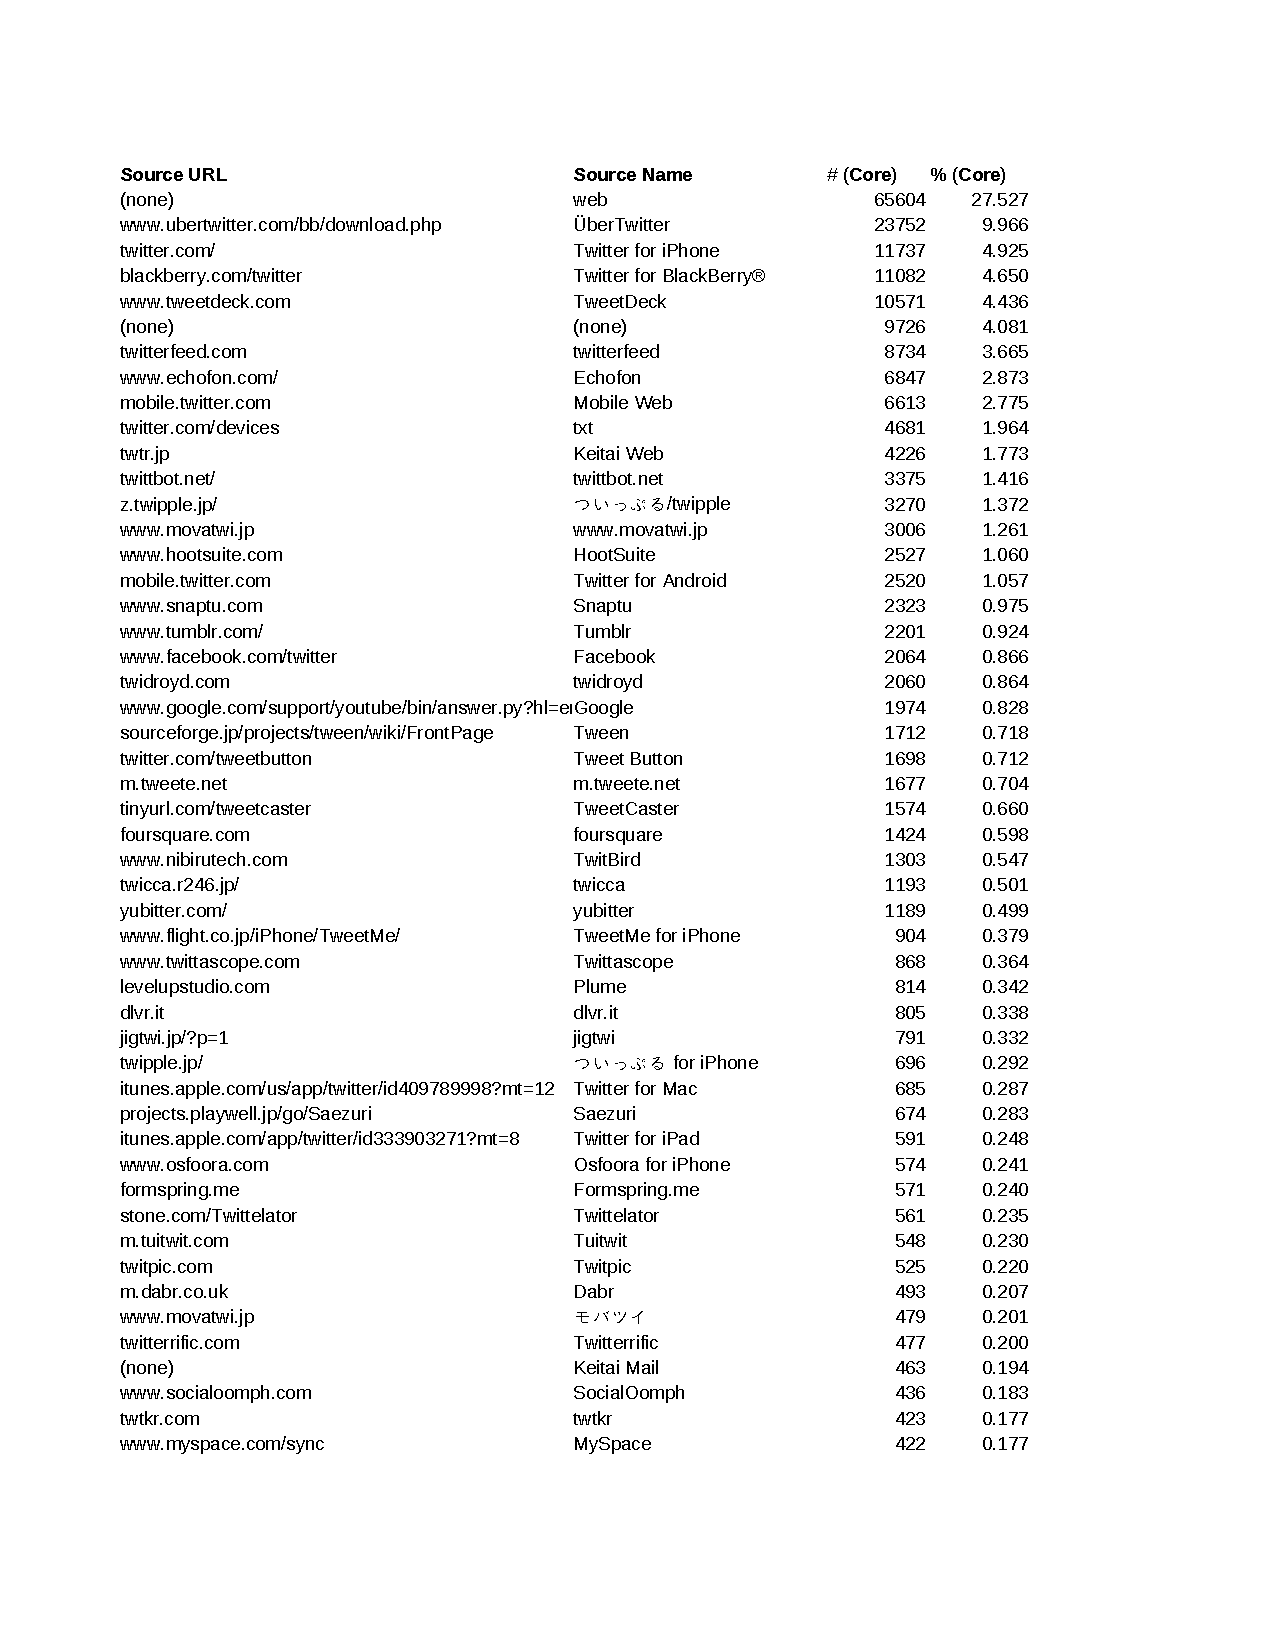
\includegraphics[width=6in,bb=0 0 612 792,keepaspectratio=true]{./sources.pdf}
% sources.pdf: 612x792 pixel, 72dpi, 21.59x27.94 cm, bb=0 0 612 792

\twocolumn
\subsection{Location}

\noindent The location attribute is a free-form value.  That is, a user can set their location to anything they want.  In order to the use the location data, we must filter and interpret these values.  The goal is to map a single geographical location to each user, but the location data is not well-formed.  Location data is sometimes not entered, non-specific (Ex: ``Under your bed"), multiple (Ex: ``NYC \& San Francisco"), or simply a non-loaction (Ex: ``Blahhhhh").\\\\
Our approach is to match each user's location against a list of known valid locations.  We are getting the list of locations from the World Cities Database (\url{http://www.maxmind.com/app/worldcities}).  World Cities has a list of all cities, regions, and countries in the world.  We first tried to match the beginning of each user's location attribute with a city.  That is, the user location could match the World Cities location exactly, or it could include characters beyond the World Cities location.  Also, capitalization is ignored.  We performed similar searches with region and country.  Overall, there were approximately 7 million users matched with a location, out of the 14.5 million total.\\\\
Some users were matched with more than one location.  For these users, we need to make a more specific location match by appending to the location string.  For example, if a user matches many cities with the name ``Springfield", we can search for ``Springfield, OR", or ``Springfield, Oregon", or ``Springfield, IL", etc.\\\\
For the users that do not match a location, we need to examine why.  We need to estimate what proportion of the non-match are non-locations, non-entered, or ill-formed.  This will be done by manual examination of a subset of the data.  We need to determine an accectable size for this subset.\\\\ 
\begin{tabular}{| l | l |}
\hline
\textbf{Match Criterion} & \textbf{Number of Users} \\ \hline
One or more cities & 8.553.747 \\ \hline
Exactly one city & 983,516 \\ \hline
One or more regions & 2,442,249 \\ \hline
Exactly one region & 1,771,560\\ \hline
One or more countries & 1,175,514 \\ \hline
Exactly one country & 1,164,406 (99.1\%) \\ \hline
\end{tabular}\\\\

\subsubsection{Other Approaches}
\noindent The Google Maps and Yahoo Maps Geocoding APIs provide translation from user-entered location strings to geographical locations.  For example, Google Maps knows that ``The City by the Bay" is San Francisco.  There are obvious advantages of this functionality, but we are unable to use these services because of strict rate-limiting.  The Geocoding API is rate-limited to 2,500 queries per day per IP address, and the Yahoo Geocoding API has a 5,000 queries per day limit.\\\\

